\documentclass{beamer}
\usepackage[utf8]{inputenc}
\usepackage{amsmath,amssymb}
\usepackage{graphicx}
\usepackage{epstopdf}
\usepackage[listings,theorems]{tcolorbox}
\usepackage{tikz}
\usepackage{pgf}
\usepackage[customcolors,shade]{hf-tikz}
\usefonttheme{serif} % default family is serif
\setbeamersize{text margin left=5mm,text margin right=5mm} 

\usetikzlibrary{positioning,shapes}
\usetikzlibrary{shapes.geometric,arrows,automata,tikzmark}
\usetikzlibrary{arrows,decorations.pathmorphing}
\tikzstyle{io} = [trapezium, trapezium left angle=70, trapezium right angle=110, minimum width=3cm, minimum height=1cm, text centered, draw=black, fill=blue!30]
\tikzstyle{process} = [rectangle, minimum width=3cm, minimum height=1cm, text centered, draw=black, fill=orange!30]
\tikzstyle{decision} = [diamond, minimum width=3cm, minimum height=1cm, text centered, draw=black, fill=green!30]
\tikzstyle{arrow} = [thick,->,>=stealth]

%Information to be included in the title page:
\title{Optimización de la estructura electrónica del átomo de O$^{6+}$}
\author{A. Mendez}
%\institute{Overleaf}
\date{\today} % It's always today!

\begin{document}
\frame{\titlepage}
%%%%%%%%%%%%%%%%%%%%%%%%%%%%%%%%%%%%%%%%%%%%%%%%%%%%%%%%%%%%%%%%%%%%%%%%
\begin{frame}
\frametitle{Minimización de $E_j$:}

\begin{tikzpicture}[remember picture, overlay]
 \tikzset{shift={(current page.center)},xshift=0cm,yshift=0cm}
 \node<1-> at (0,3.55) {\texttt{initer=60,\,maxevals=60}};
 \node<1> at (-4,1.4) {\includegraphics[width=0.35\textwidth]{figures/o6+/mod_ener/Jmin_latin.eps}};
 \node<1> at (0,1.4) {\includegraphics[width=0.35\textwidth]{figures/o6+/mod_ener/imin_latin.eps}};
 \node<1> at (4,1.4) {\includegraphics[width=0.35\textwidth]{figures/o6+/mod_ener/minspace_latin.eps}};
 \node<1> at (-2.5,-2.6) {\includegraphics[width=0.55\textwidth]{figures/o6+/mod_ener/akierp_latin.eps}};
 \node<1> at (3.75,-2.4) {\includegraphics[trim={1cm 19cm 6cm 2cm},clip,width=0.55\textwidth]{figures/o6+/mod_ener/erpmin_latin.pdf}};
\end{tikzpicture}

\end{frame}
%%%%%%%%%%%%%%%%%%%%%%%%%%%%%%%%%%%%%%%%%%%%%%%%%%%%%%%%%%%%%%%%%%%%%%%%
\begin{frame}
\frametitle{Minimización de $A_{ki}$:}

\begin{tikzpicture}[remember picture, overlay]
 \tikzset{shift={(current page.center)},xshift=0cm,yshift=0cm}
 \node<1-> at (0,3.55) {\texttt{initer=120,\,maxevals=80}};
 \node<1> at (-4,1.4) {\includegraphics[width=0.35\textwidth]{figures/o6+/mod_aki/Jmin_latin.eps}};
 \node<1> at (0,1.4) {\includegraphics[width=0.35\textwidth]{figures/o6+/mod_aki/imin_latin.eps}};
 \node<1> at (4,1.4) {\includegraphics[width=0.35\textwidth]{figures/o6+/mod_aki/minspace_latin.eps}};
 \node<1> at (-2.5,-2.6) {\includegraphics[width=0.55\textwidth]{figures/o6+/mod_aki/akierp_latin.eps}};
 \node<1> at (3.75,-2.4) {\includegraphics[trim={1cm 19cm 6cm 2cm},clip,width=0.55\textwidth]{figures/o6+/mod_aki/erpmin_latin.pdf}};
\end{tikzpicture}

\end{frame}
%%%%%%%%%%%%%%%%%%%%%%%%%%%%%%%%%%%%%%%%%%%%%%%%%%%%%%%%%%%%%%%%%%%%%%%%
\begin{frame}
\frametitle{Minimización de $E_j+A_{ki}$:}

\begin{tikzpicture}[remember picture, overlay]
 \tikzset{shift={(current page.center)},xshift=0cm,yshift=0cm}
 \node<1-> at (0,3.55) {\texttt{initer=120,\,maxevals=80}};
 \node<1> at (-4,1.4) {\includegraphics[width=0.35\textwidth]{figures/o6+/mod_ener+aki/Jmin_latin.eps}};
 \node<1> at (0,1.4) {\includegraphics[width=0.35\textwidth]{figures/o6+/mod_ener+aki/imin_latin.eps}};
 \node<1> at (4,1.4) {\includegraphics[width=0.35\textwidth]{figures/o6+/mod_ener+aki/minspace_latin.eps}};
 \node<1> at (-2.5,-2.6) {\includegraphics[width=0.55\textwidth]{figures/o6+/mod_ener+aki/akierp_latin.eps}};
 \node<1> at (3.75,-2.4) {\includegraphics[trim={1cm 19cm 6cm 2cm},clip,width=0.55\textwidth]{figures/o6+/mod_ener+aki/erpmin_latin.pdf}};
\end{tikzpicture}

\end{frame}
%%%%%%%%%%%%%%%%%%%%%%%%%%%%%%%%%%%%%%%%%%%%%%%%%%%%%%%%%%%%%%%%%%%%%%%%
%%%%%%%%%%%%%%%%%%%%%%%%%%%%%%%%%%%%%%%%%%%%%%%%%%%%%%%%%%%%%%%%%%%%%%%%
%%%%%%%%%%%%%%%%%%%%%%%%%%%%%%%%%%%%%%%%%%%%%%%%%%%%%%%%%%%%%%%%%%%%%%%%
\end{document}
